\documentclass[conference,a4paper]{IEEEtran}

% Escritura mejorada de fórmulas matemáticas
\usepackage{amsmath}

% Inserción de gráficos
\usepackage{graphicx}

% Escritura de pseudocódigo
\usepackage[kw]{pseudo}

% Escritura mejorada de tablas
\usepackage{booktabs}

% Escritura mejorada de citas bibliográficas
\usepackage{cite}

% Para cambiar el tamaño de la fuente
\usepackage{relsize}

% Macros traducidas
\def\contentsname{Índice general}
\def\listfigurename{Índice de figuras}
\def\listtablename{Índice de tablas}
\def\refname{Referencias}
\def\indexname{Índice alfabético}
\def\figurename{Fig.}
\def\tablename{TABLA}
\def\partname{Parte}
\def\appendixname{Apéndice}
\def\abstractname{Resumen}
% IEEE specific names
\def\IEEEkeywordsname{Palabras clave}
\def\IEEEproofname{Demostración}


\begin{document}

\title{Comparación de Algoritmos de Aprendizaje por Refuerzo en la Navegación de Robots Móviles: Q-Learning, Montecarlo y SARSA}

\author{
  \IEEEauthorblockN{David Fuentelsaz Rodríguez}
  \IEEEauthorblockA{
    \textit{Dpto. Ciencias de la Computación e Inteligencia Artificial}\\
    \textit{Universidad de Sevilla}\\
    Sevilla, España\\
    davfuerod@alum.us.es}
  
  \and
  
  \IEEEauthorblockN{Nombre y apellidos alumno 2}
  \IEEEauthorblockA{
    \textit{Dpto. Ciencias de la Computación e Inteligencia Artificial}\\
    \textit{Universidad de Sevilla}\\
    Sevilla, España\\
    Correos electrónicos UVUS y de contacto (si distinto)}
}

\maketitle


% Resumen
\begin{abstract}
  El objetivo principal de este trabajo es comparar tres algoritmos de aprendizaje por refuerzo: Q-Learning, Montecarlo y SARSA, en el contexto de la planificación de rutas para un robot móvil en un entorno con obstáculos. El estudio se centra en evaluar la eficiencia, la convergencia, la longitud de las rutas generadas y la capacidad de evitar colisiones de cada algoritmo al navegar hacia un destino. Los resultados obtenidos muestran que cada algoritmo presenta ventajas y desventajas específicas en diferentes aspectos del problema planteado. Q-Learning demostró una rápida convergencia y generó rutas más directas en la mayoría de los escenarios, mientras que Montecarlo ofreció una mejor exploración del espacio de estados. SARSA, por su parte, destacó en entornos altamente estocásticos debido a su enfoque de aprendizaje on-policy, aunque presentó peores resultados en general y una convergencia más lenta.\newline
  
  Estas conclusiones ofrecen una guía para la selección del algoritmo más adecuado según las características del entorno y los requisitos del sistema, y se sugieren mejoras futuras basadas en el aprendizaje transferencial y otras técnicas avanzadas.\newline
\end{abstract}


% Palabras claves
\begin{IEEEkeywords}
  Inteligencia Artificial, Aprendizaje por Refuerzo, Q-Learning, Montecarlo, SARSA, Procesos de Decisión de Markov, Entornos Estocásticos,
  Política, Exploración y Explotación.
\end{IEEEkeywords}


\section{Introducción}

El aprendizaje por refuerzo es un tipo de aprendizaje automático que se enfoca en la toma de decisiones en entornos dinámicos y no deterministas. 
En este tipo de aprendizaje, el agente interactúa con el entorno y recibe recompensas o penalizaciones en función de sus acciones.
El objetivo es maximizar las recompensas y minimizar las penalizaciones para encontrar la política óptima.\newline

Esta técnica tiene una gran variedad de aplicaciones entre las que se encuentran predicciones financieras, robótica, 
videojuegos, medicina o cualquier problema de optimización~\cite{b2}~\cite{b3}~\cite{b6}.\newline

En el contexto de nuestro trabajo, nos centraremos en la aplicación del aprendizaje por refuerzo a la planificación de rutas para robots móviles. En este problema, un robot con ruedas debe encontrar una ruta segura y eficiente en un entorno con obstáculos. Aunque este problema puede parecer simple a primera vista, la presencia de obstáculos, la estocasticidad en el efecto de las acciones 
y la necesidad de optimizar la ruta para minimizar el tiempo y los recursos hacen que sea un desafío significativo.\newline

Para evaluar la eficacia de los algoritmos de aprendizaje por refuerzo en este contexto, utilizamos tres mapas diferentes que varían en tamaño y porcentaje de obstáculos. Estos mapas nos permitirán comparar y analizar el rendimiento de los algoritmos en una variedad de escenarios.

\begin{figure}[h]
  \centering
  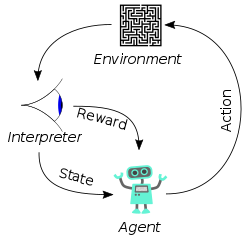
\includegraphics{Reinforcement_learning_diagram.png}
  \caption{Esquema del funcionamiento del aprendizaje por refuerzo.}
  \label{fig:Reinforcement_learning_diagram}
\end{figure}


\section{Preliminares}

En esta sección, proporcionamos una introducción a los conceptos fundamentales del aprendizaje por refuerzo,
así como una descripción de los algoritmos de aprendizaje por refuerzo que utilizaremos en nuestro trabajo.

\subsection{Conceptos clave del aprendizaje por refuerzo}

El aprendizaje por refuerzo (RL) es un tipo de aprendizaje automático que entrena al software para tomar decisiones y maximizar una recompensa en un entorno dado a través de 
un proceso de ensayo y error~\cite{b7}.\newline

Los componentes principales de un sistema de aprendizaje por refuerzo son:

\begin{itemize}
  \item \textbf{Agente}: Es la parte del sistema que toma decisiones e interactúa con el entorno. En nuestro caso, el agente es el robot móvil que busca planificar rutas en un entorno con obstáculos.
  \item \textbf{Entorno}: Es el espacio en el que el agente se mueve e interactúa. En nuestro caso, el entorno es un mapa con obstáculos.
  \item \textbf{Acción}: Una acción es la decisión tomada por el agente en un estado particular. En nuestro caso, tenemos tenemos ocho acciones que representan cada uno de los posibles movimientos que puede efectuar el robot y una 
    acción que representa que el agente permanezca en el mismo estado tras realizarla.
  \item \textbf{Recompensa}: La recompensa es la retroalimentación que el agente recibe del entorno después de tomar una acción en un estado dado. En nuestro caso, la recompensa puede ser positiva o negativa (también llamada penalización).
  \item \textbf{Política}: La política es la estrategia utilizada por el agente para seleccionar acciones en función de los estados del entorno. 
  \item \textbf{Exploración}: Es el proceso de probar nuevas acciones y recopilar información sobre el entorno. La exploración es esencial para que el agente descubra nuevas oportunidades y estrategias que podrían llevar a recompensas a largo plazo más altas.
  \item \textbf{Explotación}: Es el proceso de utilizar la información aprendida para tomar decisiones que maximicen la recompensa inmediata. La explotación es importante para que el agente obtenga la mayor recompensa posible en el momento presente.
\end{itemize}


\subsection{Descripción de los algoritmos}

A continuación, describimos los algoritmos de aprendizaje por refuerzo que utilizados en nuestro trabajo:\newline

\subsubsection{\textbf{Q-Learning}}
El algoritmo Q-Learning es un método de aprendizaje por refuerzo basado en valores que se utiliza para encontrar la política óptima de selección de acciones en un entorno determinado.
Este algoritmo es una variante del aprendizaje por refuerzo que utiliza una función de valor, denominada función Q, para determinar la mejor acción en cada estado del entorno.
No requiere un modelo del entorno y puede manejar problemas con transiciones estocásticas y recompensas sin requerir adaptaciones~\cite{b5}.

El agente explora el entorno y actualiza la tabla Q utilizando la ecuación de Bellman modificada:
\[
Q(s, a) \leftarrow Q(s, a) + \alpha [R(s, a) + \gamma \max_{a'} Q(s', a') - Q(s,a)]
\]
Donde:
\begin{itemize}
    \item \(\alpha\) es el factor de aprendizaje.
    \item \(R(s, a)\) es la recompensa inmediata por tomar la acción \(a\) en el estado \(s\).
    \item \(\gamma\) es el factor de descuento.
    \item \(s'\) es el estado siguiente al tomar la acción \(a\) en el estado \(s\).
    \item \(\max_{a'} Q(s', a')\) es el valor máximo esperado para cualquier acción posible en el estado \(s'\).\newline
\end{itemize}

Se trata de un algoritmo con un enfoque \textit{off-policy}, lo que significa que aprende la función de valor óptima independientemente de la política que el agente esté siguiendo en el momento. Q-Learning actualiza la estimación de la función Q utilizando la recompensa inmediata y el valor máximo de la función Q para el siguiente estado y acción~\cite{b1}~\cite{b4}~\cite{b5}.\newline

\textbf{Hiperparámetros en Q-Learning}
\begin{itemize}
  \item \textbf{Número de episodios:} La cantidad total de episodios que se utilizan para entrenar el algoritmo. Un mayor número de episodios puede permitir un mejor aprendizaje, aunque también incrementa el tiempo de entrenamiento.
  \item \textbf{Número de pasos máximo por episodio:} El número máximo de pasos que el agente puede tomar dentro de un solo episodio antes de que termine. Esto es útil para evitar que los episodios se alarguen indefinidamente y asegurar que el agente tenga múltiples oportunidades de aprender dentro de un tiempo razonable.
  \item \textbf{Tasa de aprendizaje (\(\alpha\)):} Controla cuánto se actualiza la función Q con nuevas experiencias. Un valor alto de \(\alpha\) permite un aprendizaje rápido pero puede causar oscilaciones, mientras que un valor bajo conduce a un aprendizaje más estable pero más lento.
  \item \textbf{Factor de descuento (\(\gamma\)):} Determina la importancia de las recompensas futuras. Un valor alto de \(\gamma\) hace que el agente valore más las recompensas futuras, mientras que un valor bajo de \(\gamma\) se centra más en las recompensas inmediatas.
  \item \textbf{Estrategia de exploración (\(\epsilon\) en \(\epsilon\)-greedy):} Controla el balance entre exploración y explotación. Un valor alto de \(\epsilon\) fomenta la exploración, mientras que un valor bajo de \(\epsilon\) fomenta la explotación de acciones conocidas.\newline
\end{itemize}


\subsubsection{\textbf{Montecarlo}}

\subsubsection{\textbf{SARSA}}
El algoritmo SARSA (State-Action-Reward-State-Action) es un algoritmo de aprendizaje por refuerzo que se utiliza para aprender una política óptima en un entorno de Markov discreto. Es bastante similar al algoritmo Q-Learning, 
aunque tiene una serie de diferencias. En primer lugar, SARSA es un algoritmo con un enfoque \textit{on-policy}, lo que significa 
que el agente aprende una política óptima mientras sigue la misma política que está aprendiendo. Este algoritmo también utiliza una tabla Q(s, a) que almacena el valor esperado de tomar la acción a en el estado s. No obstante, 
la forma en la que se actualiza Q presenta una diferencia clave respecto a Q-Learning, como se puede comprobar en la siguiente expresión:

\[
Q(s, a) \leftarrow Q(s, a) + \alpha [R(s, a) + \gamma Q(s', a') - Q(s, a)]
\]

Donde:
\begin{itemize}
    \item \(\alpha\) es el factor de aprendizaje.
    \item \(R(s, a)\) es la recompensa inmediata por tomar la acción \(a\) en el estado \(s\).
    \item \(\gamma\) es el factor de descuento.
    \item \(s'\) es el estado siguiente al tomar la acción \(a\) en el estado \(s\).
    \item \(a'\) es la acción tomada en el estado siguiente \(s'\).\newline
\end{itemize}

En este caso, se puede apreciar que la acción utilizada para actualizar la tabla Q en el siguiente estado es la seleccionada por la política actual. Al seguir un enfoque \textit{on-policy}, SARSA, por lo general, suele ser un algoritmo más lento en la convergencia a la política óptima, especialmente en entornos complejos donde se requiere la 
exploración de numerosas acciones~\cite{b4}.\newline

\textbf{Hiperparámetros en SARSA}
\begin{itemize}
  \item \textbf{Número de episodios:} La cantidad total de episodios que se utilizan para entrenar el algoritmo. Un mayor número de episodios puede permitir un mejor aprendizaje, aunque también incrementa el tiempo de entrenamiento.
  \item \textbf{Número de pasos máximo por episodio:} El número máximo de pasos que el agente puede tomar dentro de un solo episodio antes de que termine. Esto es útil para evitar que los episodios se alarguen indefinidamente y asegurar que el agente tenga múltiples oportunidades de aprender dentro de un tiempo razonable.
  \item \textbf{Tasa de aprendizaje (\(\alpha\)):} Controla cuánto se actualiza la función Q con nuevas experiencias. Un valor alto de \(\alpha\) permite un aprendizaje rápido pero puede causar oscilaciones, mientras que un valor bajo conduce a un aprendizaje más estable pero más lento.
  \item \textbf{Factor de descuento (\(\gamma\)):} Determina la importancia de las recompensas futuras. Un valor alto de \(\gamma\) hace que el agente valore más las recompensas futuras, mientras que un valor bajo de \(\gamma\) se centra más en las recompensas inmediatas.
  \item \textbf{Estrategia de exploración (\(\epsilon\) en \(\epsilon\)-greedy):} Controla el balance entre exploración y explotación. Un valor alto de \(\epsilon\) fomenta la exploración, mientras que un valor bajo de \(\epsilon\) fomenta la explotación de acciones conocidas.\newline
\end{itemize}

\subsection{Trabajos relacionados}
Para un mejor entendimiento de cómo realizar la implementación de los algoritmos, se han revisado algunos trabajos realizados:
\begin{itemize}
  \item Reinforcement Learning: An Introduction~\cite{b1}.
\end{itemize}

\section{Implementación}

En esta sección, describiremos el método implementado en nuestro trabajo. Abordaremos los siguientes dos aspectos:

\begin{itemize}
  \item Descripción del entorno de trabajo.
  \item Detalles de la implementación de los algoritmos de aprendizaje por refuerzo (Q-Learning, Montecarlo y SARSA).
\end{itemize}

\subsection{Descripción del entorno de trabajo}

En el desarrollo de este trabajo, se empleó un entorno de simulación implementado en un Jupyter Notebook. El entorno de simulación se basó en un mapa de ejemplo proporcionado en el trabajo, el cual consiste en una cuadrícula que representa el entorno en el que se moverá el robot móvil. La cuadrícula está compuesta por casillas, algunas de las cuales contienen obstáculos (representadas con unos), mientras que otras están libres de ellos (representadas con ceros).\newline

A partir del mapa de ejemplo, se generaron dos mapas adicionales para aumentar la variabilidad en los escenarios de prueba. Estos mapas proporcionaron diferentes configuraciones de entorno para evaluar el desempeño de los algoritmos de aprendizaje por refuerzo.\newline

Las casillas inicial y de destino fueron seleccionadas aleatoriamente dentro de cada mapa generado, asegurándose de que ninguna de ellas contuviera obstáculos. Esta selección aleatoria garantizó la variabilidad en los escenarios de prueba y permitió evaluar el desempeño de los algoritmos en diferentes configuraciones del entorno.\newline

En este entorno simulado, el robot móvil parte de una casilla inicial aleatoria y tiene como objetivo llegar a una casilla destino específica. Durante la simulación, el robot puede moverse entre casillas adyacentes en la cuadrícula, siguiendo una política determinada por los algoritmos de aprendizaje por refuerzo implementados. La interacción del robot con el entorno se realiza mediante acciones discretas.\newline

Este enfoque de simulación proporcionó un entorno controlado y reproducible para evaluar el rendimiento de los algoritmos de aprendizaje por refuerzo en la planificación de rutas de robots móviles. Además, permitió explorar diferentes estrategias de navegación y analizar su efectividad en la resolución de problemas de planificación de rutas en entornos con obstáculos.\newline

\begin{figure}[h]
  \centering
  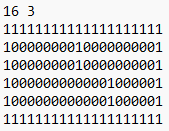
\includegraphics{Ejemplo_mapa.png}
  \caption{Ejemplo mapa generado con la casilla objetivo.}
  \label{fig:Ejemplo_mapa}
\end{figure}

\subsection{Implementación de los algoritmos de aprendizaje por refuerzo}

\textbf{Funciones auxiliares\newline}
Aquí se describen las funciones auxiliares que han sido utilizadas en la implementación de los algoritmos de aprendizaje por refuerzo.\newline

1. Método para leer el mapa de un fichero de texto

\begin{figure}[h]
  \begin{pseudo}*
    \hd{\fn{lee\_mapa}}(\textit{fichero}) \\*
    \multicolumn{2}{l}{\textbf{Entrada}: Nombre del archivo \textit{fichero}} \\*
    \multicolumn{2}{l}{\textbf{Salida}: Matriz que representa el mapa y el objetivo} \\*
    \multicolumn{2}{l}{\textbf{Algoritmo}:}\\
    Leer las líneas del archivo \textit{fichero}\\
    y convertirlas a matriz\\
    Devolver la matriz y sus dimensiones
  \end{pseudo}
  \caption{Pseudocódigo de la función \texttt{lee\_mapa}.}
  \label{fig:lee_mapa}
\end{figure}

2. Método para comprobar si una casilla contiene un obstáculo\newline

\begin{figure}[h]
  \begin{pseudo}*
    \hd{\fn{hay\_colision}}(\textit{estado}) \\*
    \multicolumn{2}{l}{\textbf{Entrada}: Casilla en la que se encuentra el robot \textit{estado}} \\*
    \multicolumn{2}{l}{\textbf{Salida}: Valor booleano que indica si hay colisión} \\*
    \multicolumn{2}{l}{\textbf{Algoritmo}:} \\
    Verificar si hay un obstáculo en \textit{estado} \\
    Devolver \textbf{true} si hay colisión, \textbf{false} en caso contrario
  \end{pseudo}
  \caption{Pseudocódigo del método \texttt{hay\_colision}.}
  \label{fig:hay_colision}
\end{figure}

3. Método para aplicar una acción en un estado

\begin{figure}[h]
  \begin{pseudo}*
    \hd{\fn{aplica\_accion}}(\textit{estado}, \textit{accion}) \\*
    \multicolumn{2}{l}{\textbf{Entrada}: \textit{estado} y \textit{accion}} \\*
    \multicolumn{2}{l}{\textbf{Salida}: Nuevo \textit{estado}} \\*
    \multicolumn{2}{l}{\textbf{Algoritmo}:}\\
    \textbf{Si} hay colisión \textbf{entonces} \\
    \> Devolver \textit{estado} \\
    $x, y \leftarrow$ Coordenadas de \textit{estado} \\
    \textbf{Si} \textit{accion} es norte \textbf{entonces} \\
    \> $y \leftarrow y + 1$ \\
    \textbf{Si no, si} \textit{accion} es sur \textbf{entonces} \\
    \> $y \leftarrow y - 1$ \\
    \textbf{Si no, si} \textit{accion} es este \textbf{entonces} \\
    \> $x \leftarrow x + 1$ \\
    \textbf{Si no, si} \textit{accion} es oeste \textbf{entonces} \\
    \> $x \leftarrow x - 1$ \\
    \textbf{Sino, si} \textit{accion} es noreste \textbf{entonces} \\
    \> $x, y \leftarrow x + 1, y + 1$ \\
    \textbf{Si no, si} \textit{accion} es sureste \textbf{entonces} \\
    \> $x, y \leftarrow x + 1, y - 1$ \\
    \textbf{Si no, si} \textit{accion} es suroeste \textbf{entonces} \\
    \> $x, y \leftarrow x - 1, y - 1$ \\
    \textbf{Si no, si} \textit{accion} es noroeste \textbf{entonces} \\
    \> $x, y \leftarrow x - 1, y + 1$ \\
    Devolver $(x, y)$ como nuevo \textit{estado}
  \end{pseudo}
  \caption{Pseudocódigo de \texttt{aplica\_accion}.}
  \label{fig:aplica_accion}
\end{figure}

4. Método para obtener los estados libres de obstáculos

\begin{figure}[h]
  \begin{pseudo}*
    \hd{\fn{estados\_sin\_obstaculos}}() \\*
    \multicolumn{2}{l}{\textbf{Salida}: Lista de estados sin obstáculos} \\*
    \multicolumn{2}{l}{\textbf{Algoritmo}:}\\
    Inicializar una lista vacía llamada \textit{estados\_sin\_obstaculos} \\
    \fn{Para cada} estado \textit{en} \textit{nav\_estados} \fn{hacer} \\
    \> \fn{Si no} \fn{hay\_colision}(estado) \fn{entonces} \\
    \> \> Agregar el estado a la lista \textit{estados\_sin\_obstaculos} \\
    Devolver la lista \textit{estados\_sin\_obstaculos}
  \end{pseudo}
  \caption{Pseudocódigo detallado de \texttt{estados\_sin\_obstaculos}.}
  \label{fig:estados_sin_obstaculos}
\end{figure}

Siendo \textit{nav\_estados} la variable global con todos los estados del entorno.\newline

5. Método para obtener los posibles desvíos del agente al realizar una acción

\begin{figure}[h]
  \begin{pseudo}*
    \hd{\fn{obtiene\_posibles\_errores}}(\textit{accion}) \\*
    \multicolumn{2}{l}{\textbf{Entrada}: \textit{accion}} \\*
    \multicolumn{2}{l}{\textbf{Salida}: Lista de posibles acciones erróneas} \\*
    \multicolumn{2}{l}{\textbf{Algoritmo}:}\\
    \textbf{Si} \textit{accion} es norte \textbf{entonces} \\
    \> \textit{errores} $\leftarrow$ ['NE', 'NO'] \\
    \textbf{Si no, si} \textit{accion} es sur \textbf{entonces} \\
    \> \textit{errores} $\leftarrow$ ['SE', 'SO'] \\
    \textbf{Si no, si} \textit{accion} es este \textbf{entonces} \\
    \> \textit{errores} $\leftarrow$ ['NE', 'SE'] \\
    \textbf{Si no, si} \textit{accion} es oeste \textbf{entonces} \\
    \> \textit{errores} $\leftarrow$ ['NO', 'SO'] \\
    \textbf{Si no, si} \textit{accion} es noreste \textbf{entonces} \\
    \> \textit{errores} $\leftarrow$ ['N', 'E'] \\
    \textbf{Si no, si} \textit{accion} es noroeste \textbf{entonces} \\
    \> \textit{errores} $\leftarrow$ ['N', 'O'] \\
    \textbf{Si no, si} \textit{accion} es sureste \textbf{entonces} \\
    \> \textit{errores} $\leftarrow$ ['S', 'E'] \\
    \textbf{Si no, si} \textit{accion} es suroeste \textbf{entonces} \\
    \> \textit{errores} $\leftarrow$ ['S', 'O'] \\
    \textbf{Si no} \\
    \> \textit{errores} $\leftarrow$ [] \\
    Devolver \textit{errores}
  \end{pseudo}
  \caption{Pseudocódigo de \texttt{obtiene\_posibles\_errores}.}
  \label{fig:obtiene_posibles_errores}
\end{figure}


6. Método para escoger una acción a partir de la política \(\epsilon-greedy\)\
  
\begin{figure}[h]
  \begin{pseudo}*
    \hd{\fn{escoger\_accion}}(\textit{estado}, \textit{epsilon}) \\*
    \multicolumn{2}{l}{\textbf{Entrada}: Estado \textit{estado} y valor de epsilon \textit{epsilon}} \\*
    \multicolumn{2}{l}{\textbf{Salida}: Acción seleccionada} \\*
    \multicolumn{2}{l}{\textbf{Algoritmo}:}\\
    \textbf{Si} \textit{estado} no está en la tabla Q \textbf{entonces} \\
    \> Inicializar los valores de \textit{estado} a cero en la tabla Q \\
    \\
    \textbf{Si} un número aleatorio entre 0 y 1 es menor que \textit{epsilon}\\
    \> \textbf{Seleccionar} una acción aleatoria \\
    \textbf{Si no} \\
    \> \textbf{Seleccionar} la mejor acción conocida \\
    \\
    Devolver la acción seleccionada
  \end{pseudo}
  \caption{Pseudocódigo de \texttt{escoger\_accion}.}
  \label{fig:escoger_accion}
\end{figure}

7. Método para obtener la política a partir de los valores de la tabla Q\newline\newline\newline\newline\newline\newline\newline\newline

\begin{figure}[h]
  \begin{pseudo}*
    \hd{\fn{obtener\_politica}}(\textit{Q}) \\*
    \multicolumn{2}{l}{\textbf{Entrada}: Tabla \textit{Q}} \\*
    \multicolumn{2}{l}{\textbf{Salida}: Política basada en \textit{Q}} \\*
    \multicolumn{2}{l}{\textbf{Algoritmo}:} \\
    Inicializar \textit{politica} como diccionario vacío \\
    \textbf{Para cada} estado \textit{en} nav\_estados \textbf{hacer} \\
    \> \textbf{Si} estado \textit{está en} Q\_table \textbf{entonces} \\
    \> \> \textit{politica[estado]} $\leftarrow$ índice de max(\textit{Q\_table[estado]}) \\
    \> \textbf{Sino} \\
    \> \> \textit{politica[estado]} $\leftarrow$ 0 \\
    \textbf{Retornar} \textit{politica}
  \end{pseudo}
  \caption{Pseudocódigo de la función \texttt{obtener\_politica}.}
  \label{fig:obtener_politica}
\end{figure}

8. Método para obtener la recompensa de aplicar una acción a un estado

\begin{figure}[h]
  \begin{pseudo}*
    \hd{\fn{obtiene\_recompensa}}(\textit{estado}, \textit{accion}) \\*
    \multicolumn{2}{l}{\textbf{Entrada}: Estado actual \textit{estado}, acción a tomar \textit{accion}} \\*
    \multicolumn{2}{l}{\textbf{Salida}: Recompensa correspondiente} \\*
    \multicolumn{2}{l}{\textbf{Algoritmo}:} \\
    \textit{x, y} $\leftarrow$ \textit{estado} \\
    \textbf{Si} \textit{estado} es igual a \textit{destino} \textbf{entonces} \\
    \> devolver \textit{recompensa\_objetivo\_alcanzado} \\
    \textbf{Si} hay colisión en \textit{estado} \textbf{entonces} \\
    \> devolver -\textit{penalizacion\_colision} \\
    \textbf{Si} \textit{accion} es igual a 'esperar' \textbf{entonces} \\
    \> devolver -\textit{penalizacion\_esperar} \\
    \textbf{Para cada} \textit{accion\_error} \\ en obtiene\_posibles\_errores(\textit{accion}) \textbf{hacer} \\
    \> \textit{estado\_vecino} $\leftarrow$ aplica\_accion(\textit{estado}, \textit{accion\_error}) \\
    \> \textbf{Si} hay colisión en \textit{estado\_vecino} \textbf{entonces} \\
    \> \> devolver -\textit{penalizacion\_casilla\_adyacente\_obstaculo} \\
  \end{pseudo}
  \caption{Pseudocódigo de la función \texttt{obtiene\_recompensa}.}
  \label{fig:obtiene_recompensa}
  \vspace{0.5cm} 
  En este caso, \textit{recompensa\_objetivo\_alcanzado}, \textit{penalizacion\_colision}, \textit{penalizacion\_esperar} y \textit{penalizacion\_casilla\_adyacente\_obstaculo}
son variables globales que se usan en el método para definir el valor de la recompensa en diferentes situaciones.\newline

Tras presentar todas las funciones auxiliares utilizadas en la implementación de los algoritmos, procedemos a detallar la implementación de Q-Learning, Montecarlo y SARSA.\newline 

\end{figure}


\textbf{Q-Learning\newline}

En primer lugar, nos encontramos con el algoritmo de Q-Learning. Los valores de los hiperparámetros se han seleccionado de manera que optimicen el rendimiento del algoritmo. 
No obstante, en la siguiente sección se detallarán los experimentos y pruebas realizadas.\newline\newline\newline

\begin{figure}[h]
  \begin{pseudo}[compact]
    \textbf{Q-Learning}: \\
    Inicializar $Q$ como diccionario vacío \\
    Parámetros: $\alpha = 0.2$, $\gamma = 0.9$, $\epsilon = 0.3$, \\ $epocas = 5000$, $max\_pasos = 100$ \\
    Para cada época: \\
    \> Estado aleatorio sin obstáculos \\
    \> Para cada paso: \\
    \> \> \textit{accion\_index} $\leftarrow$ escoger\_accion(\textit{estado}, $\epsilon$) \\
    \> \> \textit{accion} $\leftarrow$ nav\_acciones[\textit{accion\_index}] \\
    \> \> Aplicar acción, obtener nuevo estado y recompensa \\
    Si \textit{estado} no está en \textit{Q\_table} entonces \\+
      Inicializar \textit{Q\_table}[\textit{estado}] con ceros \\-
    \textbf{Fin Si} \\
    Si \textit{nuevo\_estado} no está en \textit{Q\_table} entonces \\+
      Inicializar \textit{Q\_table}[\textit{nuevo\_estado}] con ceros \\-
    \textbf{Fin Si} \\
    \textit{mejor\_accion\_nueva} $\leftarrow$ max\textit{Q\_table}[\textit{nuevo\_estado}] \\
    \textit{Q\_table}[\textit{estado}][\textit{accion}] $\leftarrow$ \textit{Q\_table}[\textit{estado}][\textit{accion}] + \\
    \> \textit{alpha} * (\textit{recompensa} + \textit{gamma} * \textit{mejor\_accion\_nueva}\\
    \> - \textit{Q\_table}[\textit{estado}][\textit{accion}])\\
    \> Si estado destino o terminal, terminar \\
  \end{pseudo}
  \caption{Pseudocódigo del algoritmo Q-Learning.}
  \label{fig:q-learning}
\end{figure}



\textbf{SARSA\newline}

A continuación se muestran los detalles de la implementación realizada del algoritmo SARSA. De igual manera que en Q-Learning, el valor de los hiperparámetros
se han seleccionado de manera que optimicen el rendimiento del algoritmo. 

\begin{figure}[!h]
  \begin{minipage}{\linewidth}
    \begin{pseudo}[compact]
      \textbf{SARSA}: \\
      Inicializar $Q\_table$ como diccionario vacío \\
      Parámetros: $\alpha = 0.1$, $\gamma = 0.9$, $\epsilon = 0.3$, \\ $num\_episodios = 100000$, $max\_pasos = 100$ \\
      Para cada episodio: \\
      \> Estado aleatorio sin obstáculos \\
      \> \textit{accion\_index} $\leftarrow$ escoger\_accion(\textit{estado}, $\epsilon$) \\
      \> \textit{accion} $\leftarrow$ nav\_acciones[\textit{accion\_index}] \\
      \> Para cada paso: \\
      \> \> Aplicar acción, obtener nuevo estado y recompensa \\
      \> \> \textit{nueva\_accion\_index} $\leftarrow$ \\
      \> \> \> escoger\_accion(\textit{nuevo\_estado}, $\epsilon$) \\
      \> \> \textit{nueva\_accion} $\leftarrow$ nav\_acciones[\textit{nueva\_accion\_index}] \\
      Si \textit{estado} no está en \textit{Q\_table} entonces \\+
      Inicializar \textit{Q\_table}[\textit{estado}] con ceros \\-
    \end{pseudo}
  \end{minipage}
  \caption{Pseudocódigo del algoritmo SARSA (Parte 1).}
  \label{fig:sarsa1}
\end{figure}


\begin{figure}
  \begin{minipage}{\linewidth}
  \begin{pseudo}
  \textbf{Fin Si} \\
  Si \textit{nuevo\_estado} \textnormal{no está en} \textit{Q\_table} entonces \\+
    Inicializar \textit{Q\_table}[\textit{nuevo\_estado}] con ceros \\-
  \textbf{Fin Si} \\
  \textit{Q\_table}[\textit{estado}][\textit{accion}] $\leftarrow$ \textit{Q\_table}[\textit{estado}][\textit{accion}] + \\
  \> $\alpha \cdot (\textit{recompensa} + $ \\
  \> $\gamma \cdot \textit{Q\_table}[\textit{nuevo\_estado}][\textit{nueva\_accion}] -$ \\
  \> $\textit{Q\_table}[\textit{estado}][\textit{accion}])$ \\
  \> \textit{estado} $\leftarrow$ \textit{nuevo\_estado} \\
  \> \textit{accion} $\leftarrow$ \textit{nueva\_accion} \\
  \> Si \textit{estado} == destino, terminar \\
  \end{pseudo}
  \end{minipage}
  \caption{Pseudocódigo del algoritmo SARSA (Parte 2).}
  \label{fig:sarsa2}
  \vspace{0.5cm} 
  En esta ocasión, al actualizar los valores de la tabla Q, el robot tiene en cuenta la política que está siguiendo. Esto es debido a su enfoque \textit{on-policy}, diferenciándolo de esta manera del algoritmo de Q-Learning.\newline
\end{figure}



\section{Pruebas y experimentación}
En esta sección, se detallan los experimentos realizados y los resultados obtenidos al aplicar tres algoritmos de aprendizaje por refuerzo (Q-Learning, Montecarlo y SARSA) 
en el contexto de la planificación de rutas por parte de un robot móvil.

\subsection{Experimentos realizados}

Para llevar a cabo los experimentos, se diseñaron tres mapas de prueba, cada uno con un tamaño diferente, un porcentaje distinto de obstáculos y 
una casilla objetivo única. La posición inicial del robot se selecciona de manera aleatoria en cada experimento. 
El objetivo es evaluar la capacidad del agente para planificar una ruta segura hacia el objetivo, evitando colisionar con los obstáculos presentes en el entorno. 
Se espera que el agente se mueva por zonas alejadas de los pasillos para maximizar la seguridad durante la navegación.\newline

A continuación, se presentan los resultados obtenidos de los experimentos realizados con cada uno de los algoritmos de aprendizaje por refuerzo. Se probaron diferentes configuraciones en los hiperparámetros de cada algoritmo para evaluar su rendimiento en una variedad de escenarios.\newline

\subsubsection{\textbf{Q-Learning}}

Como se describió en la sección de \textit{Implementación}, los hiperparámetros utilizados para ajustar el rendimiento del algoritmo Q-Learning son los siguientes:\newline

Tasa de aprendizaje($\alpha$) = 0.2, Factor de descuento($\gamma$) = 0.9, Tasa de exploración($\epsilon$) = 0.3,  Épocas de entrenamiento = 5000, Máximo de pasos por episodio = 100\newline

Se optó por valores bajos de $\alpha$ y $\epsilon$ para priorizar la explotación de la mejor acción conocida y permitir que el agente aprenda de manera gradual, evitando posibles desbordamientos en los resultados que podrían surgir de un aprendizaje demasiado rápido.
Adicionalmente, probamos con un valor alto de $\gamma$ para que el agente priorizara las recompensas futuras sobre las inmediatas.\newline

A continuación, se presentan los resultados obtenidos en cada uno de los mapas de prueba:

\begin{figure}[h]
  \centering
  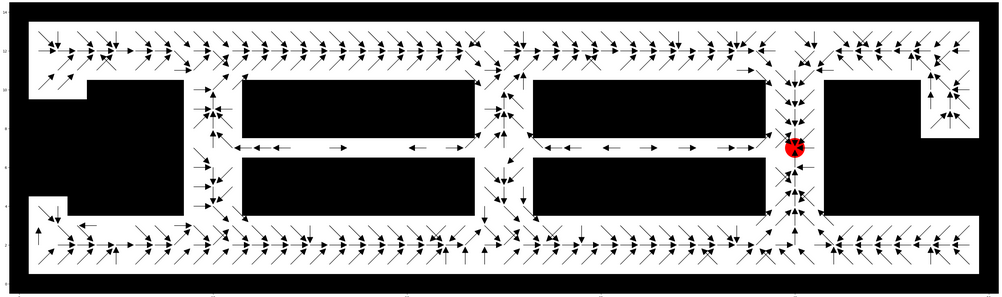
\includegraphics[scale=0.33]{resultado_qlearning_mapa_1}
  \caption{Resultados Q-Learning mapa 1}
  \label{fig:resultado_qlearning_mapa_1}
\end{figure}

\begin{figure}[h]
  \centering
  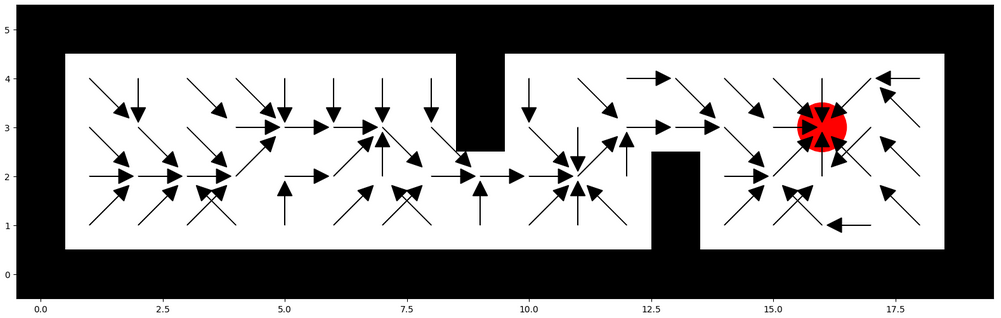
\includegraphics[scale=0.33]{resultado_qlearning_mapa_2}
  \caption{Resultados Q-Learning mapa 2}
  \label{fig:resultado_qlearning_mapa_2}
\end{figure}

\begin{figure}[h]
  \centering
  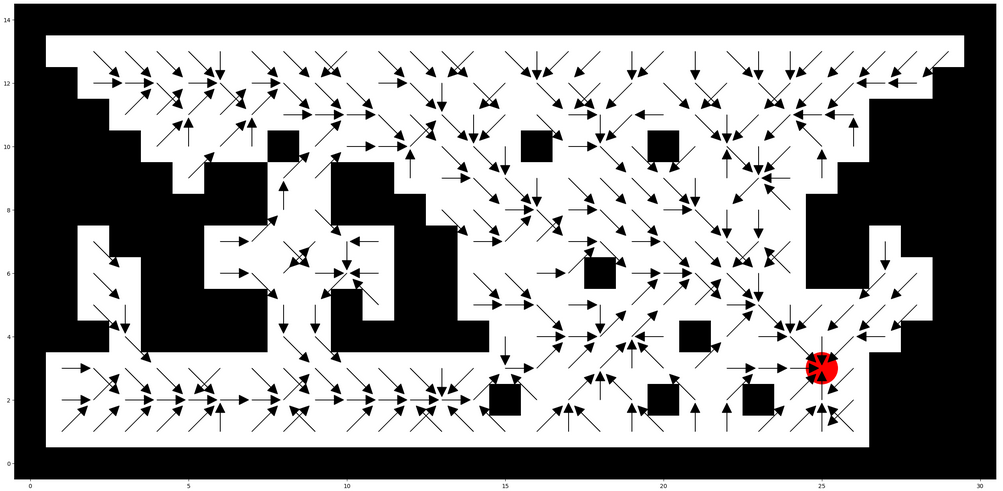
\includegraphics[scale=0.33]{resultado_qlearning_mapa_3}
  \caption{Resultados Q-Learning mapa 3}
  \label{fig:resultado_qlearning_mapa_3}
\end{figure}

Las imágenes de las rutas diseñadas por el robot en cada uno de los tres mapas muestran resultados muy satisfactorios por varias razones.
En primer lugar, el robot ha sido capaz de generar rutas cortas y directas, minimizando el tiempo y los recursos necesarios para alcanzar el objetivo.
Además, el robot ha demostrado una habilidad consistente para evitar colisiones con los obstáculos presentes en los mapas, incluso en aquellos con una mayor densidad de obstáculos. Finalmente, se destaca la robustez del algoritmo, 
ya que los resultados han sido satisfactorios en todos los mapas, a pesar de las variaciones en el tamaño, la densidad de obstáculos y la posición del estado objetivo.\newline

Por otro lado, tras realizar numerosas pruebas con variaciones en el valor de los hiperparámetros, llegamos a la conclusión de que las modificaciones en los valores de la tasa de aprendizaje, el factor de descuento y la tasa de exploración no producían cambios significativos en los resultados,
e incluso en algunos casos se observaron pequeñas mejoras. No obstante, se pudo verificar que al reducir significativamente el \textit{número de épocas de entrenamiento} 
del algoritmo, los resultados fueron mucho peores. Por ejemplo, al establecer el número de épocas en 1000,
estos son los resultados obtenidos en cada uno de los mapas:

\begin{figure}[h]
  \centering
  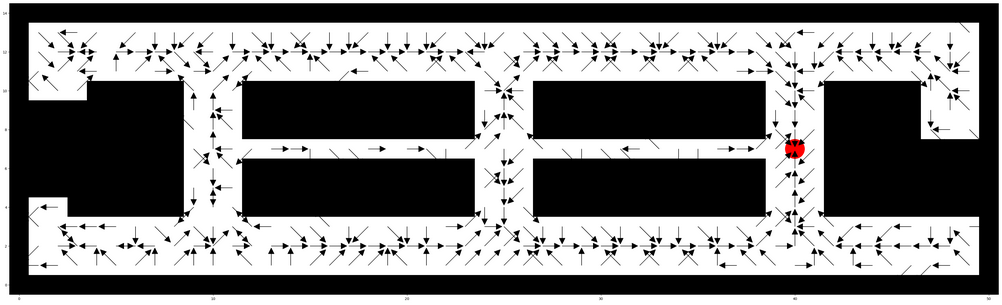
\includegraphics[scale=0.33]{resultado_2_qlearning_mapa_1}
  \caption{Resultados Q-Learning mapa 1 tras modificar el número de épocas}
  \label{fig:resultado_2_qlearning_mapa_1}
\end{figure}

\begin{figure}[h]
  \centering
  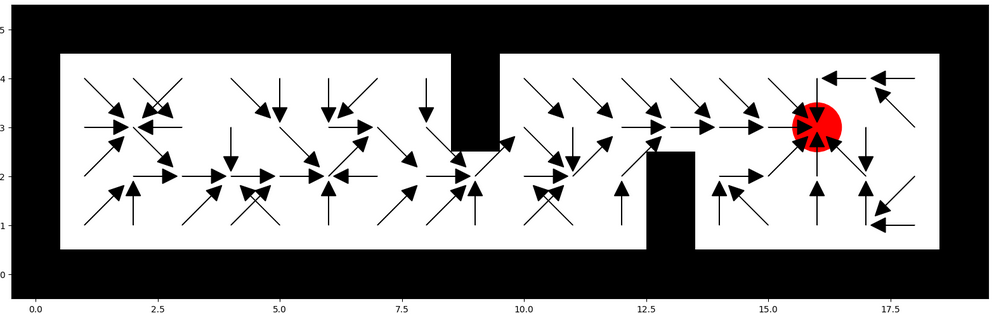
\includegraphics[scale=0.33]{resultado_2_qlearning_mapa_2}
  \caption{Resultados Q-Learning mapa 2 tras modificar el número de épocas}
  \label{fig:resultado_2_qlearning_mapa_2}
\end{figure}

\begin{figure}[h]
  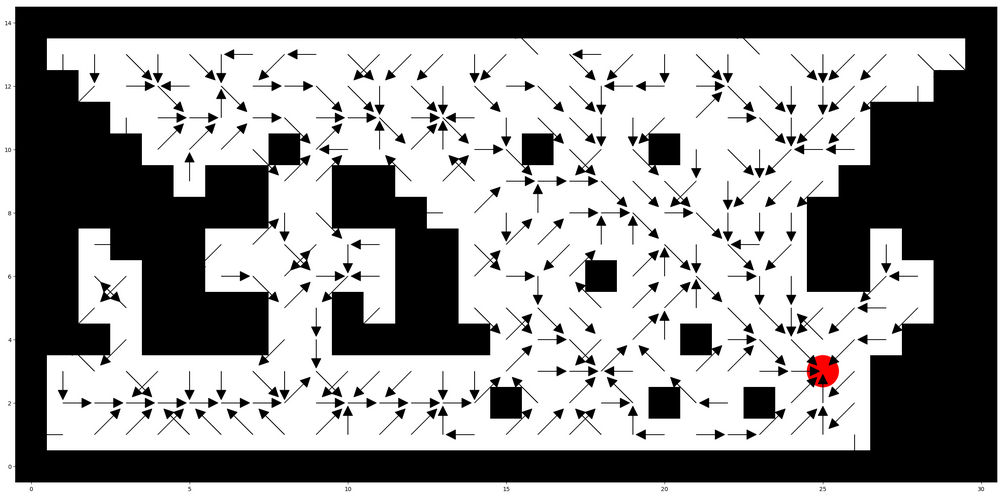
\includegraphics[scale=0.33]{resultado_2_qlearning_mapa_3}
  \caption{Resultados Q-Learning mapa 3 tras modificar el número de épocas}
  \label{fig:resultado_2_qlearning_mapa_3}
  \vspace{0.5cm}
  Como se puede apreciar, los resultados no son tan satisfactorios, ya que el robot colisiona con los obstáculos en ciertas ocasiones y no suele seleccionar la ruta más eficiente para llegar a la casilla objetivo. 
  Este empeoramiento de los resultados es más notorio en los mapas 1 y 3, lo cual tiene sentido porque, al ser mapas más grandes, requieren un mayor número de épocas de entrenamiento para que el agente aprenda la política óptima.\newline
\end{figure}

\subsubsection{\textbf{SARSA}}

En la implementación del algoritmo SARSA, los valores de los hiperparámetros se ajustaron según el mapa. En el mapa 2 (el más simple de todos), aumentamos la tasa de aprendizaje a 0.5 para que el agente pudiera aprender rápidamente sin una excesiva preocupación por desbordamientos en los valores Q.
Además, reducimos el factor de descuento a 0.5, ya que en un mapa más pequeño las recompensas futuras no son tan importantes como las inmediatas, dado que el objetivo está más cerca.
Mantenemos el valor de epsilon muy bajo, en 0.1, pues la simpleza del mapa permite que este pueda ser explorado completamente de manera rápida.\newline

En los otros dos mapas, al ser entornos más complejos, disminuimos la tasa de aprendizaje y aumentamos tanto el factor de descuento como la tasa de exploración. Estas modificaciones permiten que el agente explore más y valore mejor las recompensas a largo plazo, necesarios en escenarios más complicados.\newline

Finalmente, es importante destacar que el número de episodios de entrenamiento es significativamente mayor que en Q-Learning. Esto se debe a que SARSA, al tener un enfoque \textit{on-policy}, normalmente converge más lentamente hacia una política óptima, especialmente cuando la estrategia de exploración no se 
maneja adecuadamente~\cite{b4}. Por ello, consideramos necesario aumentar el número de iteraciones del algoritmo.\newline

A continuación, se presentan los resultados obtenidos en cada uno de los mapas de prueba:\newline

\begin{figure}[h]
  \centering
  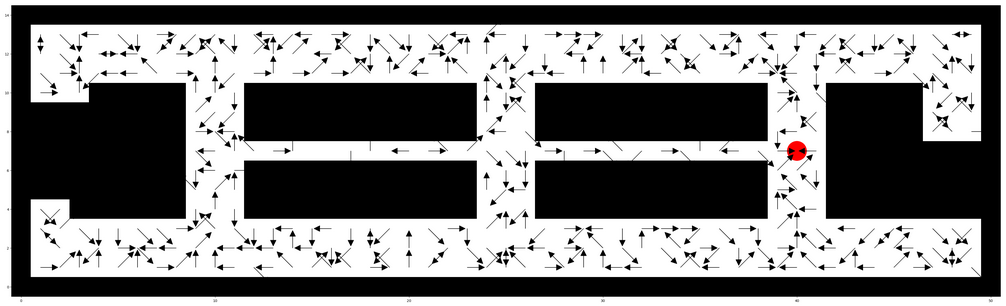
\includegraphics[scale=0.33]{resultado_sarsa_mapa_1}
  \caption{Resultados SARSA mapa 1}
  \label{fig:resultado_sarsa_mapa_1}
\end{figure}

\begin{figure}[h]
  \centering
  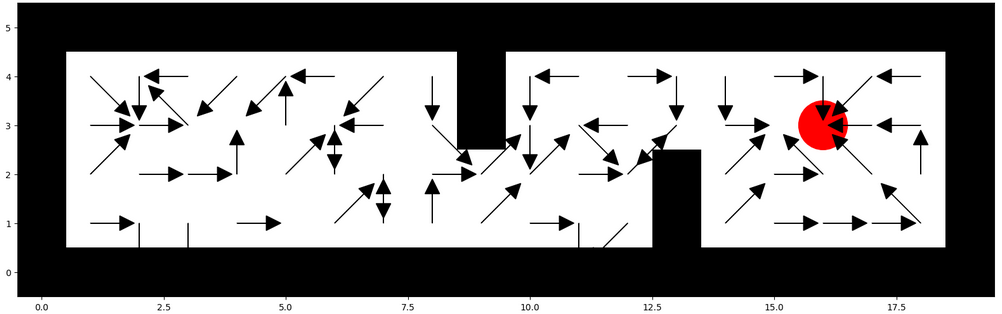
\includegraphics[scale=0.33]{resultado_sarsa_mapa_2}
  \caption{Resultados SARSA mapa 2}
  \label{fig:resultado_sarsa_mapa_2}
\end{figure}

\begin{figure}[h]
  \centering
  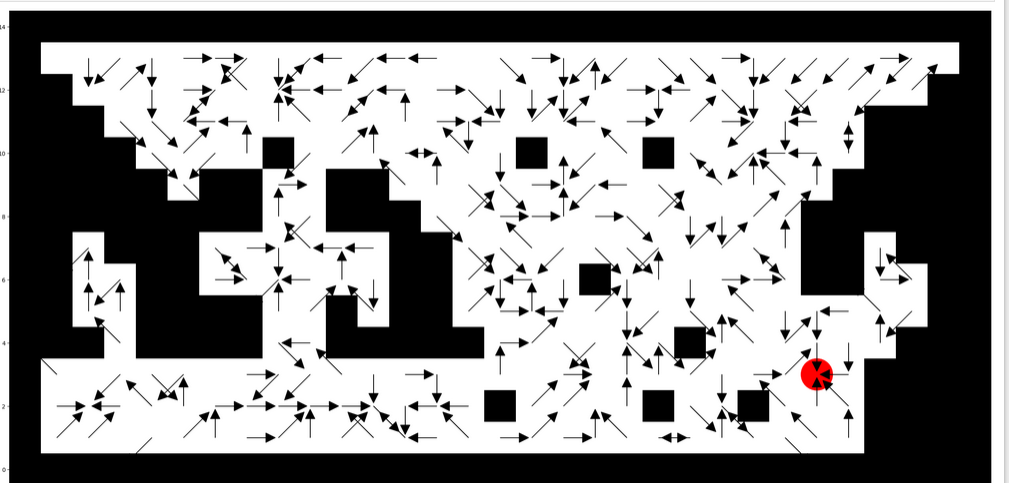
\includegraphics[scale=0.33]{resultado_sarsa_mapa_3}
  \caption{Resultados SARSA mapa 3}
  \label{fig:resultado_sarsa_mapa_3}
\end{figure}

Tras implementar y ejecutar el algoritmo SARSA con los hiperparámetros descritos anteriormente, los resultados obtenidos fueron comparativamente inferiores a los logrados con Q-Learning y Montecarlo. 
En primer lugar, las rutas generadas por SARSA fueron, en promedio, más largas y menos directas. Además, se observó que el agente colisionó con obstáculos con mayor frecuencia, lo que indica que el robot no aprendió completamente a esquivar los obstáculos. Por último, SARSA mostró una convergencia más lenta hacia una política óptima. 
A pesar del aumento en el número de episodios de entrenamiento, la política aprendida no alcanzó el mismo nivel de eficacia que las aprendidas con los otros algoritmos.\newline

Una observación interesante es que, a diferencia de Q-Learning, los hiperparámetros en este algoritmo tienen una mayor relevancia en su ejecución, evidenciándose caídas en el rendimiento cuando se probaban con valores alejados a los explicados con anterioridad.

\section{Conclusiones}

En este trabajo, se ha llevado a cabo una comparación exhaustiva de tres algoritmos de aprendizaje por refuerzo (Q-Learning, Montecarlo y SARSA) aplicados a la planificación de rutas para un robot móvil en un entorno con obstáculos.
Se diseñaron y probaron tres mapas diferentes, variando en tamaño y densidad de obstáculos, para evaluar la capacidad de cada algoritmo para generar rutas seguras y eficientes. Los resultados obtenidos se analizaron 
en términos de la longitud de las rutas generadas, la frecuencia de colisiones y la convergencia hacia políticas óptimas.\newline

Los experimentos demostraron que Q-Learning y Montecarlo proporcionaron resultados superiores en comparación con SARSA. Q-Learning generó rutas más cortas y directas, y mostró una alta 
capacidad para evitar colisiones incluso en entornos complejos. Montecarlo también tuvo un buen rendimiento, aunque su convergencia fue más lenta en comparación con Q-Learning. Por otro lado,
SARSA presentó rutas más largas y menos directas, con una mayor frecuencia de colisiones y una convergencia más lenta, incluso con un mayor número de episodios de entrenamiento.
Además, los resultados de SARSA fueron más sensibles a los valores de los hiperparámetros, mostrando una caída significativa en el rendimiento cuando se alejaban de los valores óptimos.\newline

Las conclusiones principales de este trabajo indican que Q-Learning es el algoritmo más robusto y eficiente para la tarea de planificación de rutas en entornos con obstáculos, seguido de Montecarlo. 
SARSA, aunque conceptualmente sólido, mostró limitaciones en términos de eficiencia y robustez en comparación con los otros dos algoritmos. La sensibilidad de SARSA a los hiperparámetros sugiere que 
requiere una mayor afinación para obtener resultados competitivos.\newline

Como ideas de mejora y trabajo futuro, se podría investigar la combinación de estos algoritmos con técnicas de aprendizaje profundo, como Deep Q-Learning, para manejar entornos más complejos y
de mayor dimensionalidad. Además, se podría explorar la integración de mecanismos de aprendizaje transferencial para permitir al robot aplicar conocimientos previos a nuevos entornos, mejorando
así su capacidad de generalización y adaptabilidad.

\begin{figure}[h!]
  \begin{thebibliography}{99}
  \bibitem{b1} Richard S. Sutton y Andrew G. Barto. Reinforcement Learning: An Introduction.
  MIT Press, 2018.
  \bibitem{b2}  Russell, Stuart and Norvig, Peter. Artificial Intelligence: A Modern Approach
  (2010). Chapter 21.
  \bibitem{b3} https://www.aprendemachinelearning.com/aprendizaje-por-refuerzo/
  \bibitem{b4} https://www.javatpoint.com/sarsa-reinforcement-learning
  \bibitem{b5} https://es.wikipedia.org/wiki/Q-learning
  \bibitem{b6} https://www.codificandobits.com/curso/aprendizaje-por-refuerzo-nivel-basico/2-ejemplos-reales-aplicacion-aprendizaje-por-refuerzo/
  \bibitem{b7} https://aws.amazon.com/es/what-is/reinforcement-learning/

  \end{thebibliography}
  \caption{Referencias bibliográficas.}
  \label{fig:bibliography}
  \end{figure}
  


\end{document}
